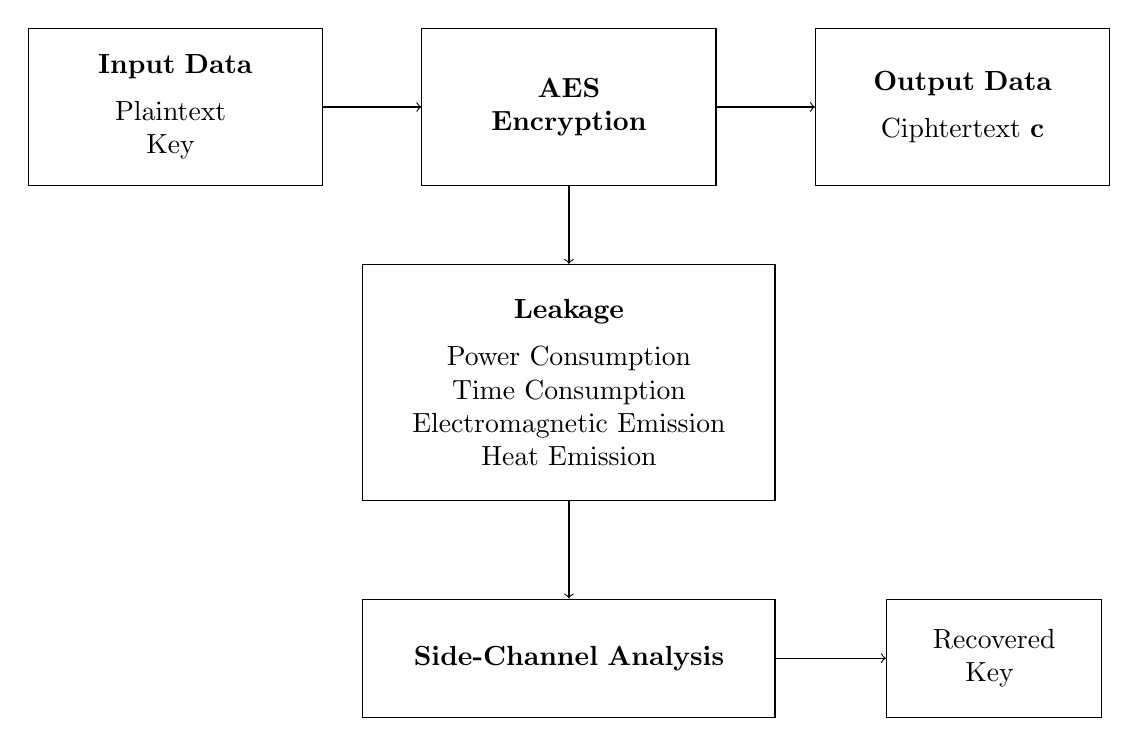
\begin{tikzpicture}%[trim left=5cm]
        \node[text width=3.5cm, align=center] (in) at (0,0) [draw,minimum width=1.5cm,minimum height=2cm] {\textbf{Input Data} \\ \vspace{0.5em} Plaintext $\pp$ \\ Key $\kk$};
        \node[text width=3.5cm, align=center] (aes) at (5,0) [draw,minimum width=1.5cm,minimum height=2cm] {\textbf{AES \\ Encryption}};
        \node[text width=3.5cm, align=center] (out) at (10,0) [draw,minimum width=1.5cm,minimum height=2cm] {\textbf{Output Data} \\ \vspace{0.5em} Ciphtertext $\mathbf{c}$};

        \node[text width=5cm, align=center] (leak) at (5,-3.5) [draw,minimum width=1.5cm,minimum height=3cm] {\textbf{Leakage} \\ \vspace{0.5em} Power Consumption \\  Time Consumption \\ Electromagnetic Emission \\ Heat Emission};
        \node[text width=5cm, align=center] (sca) at (5,-7) [draw,minimum width=1.5cm,minimum height=1.5cm] {\textbf{Side-Channel Analysis}};
        \node[text width=2.5cm, align=center] (k) at (10.4,-7) [draw,minimum width=1.0cm,minimum height=1.5cm] {Recovered \\ Key $\kk$};

        \draw[->] (in) -- (aes) node[midway,left] {};
        \draw[->] (aes) -- (out) node[midway,left] {};
        \draw[->] (aes) -- (leak) node[midway,left] {};
        \draw[->] (leak) -- (sca) node[midway,left] {};
        \draw[->] (sca) -- (k) node[midway,left] {};
\end{tikzpicture}
